\documentclass[11pt,a4paper]{article}
\usepackage{amsmath, graphicx, geometry, float}
\usepackage{hyperref, caption, subcaption}
\usepackage{typearea}

\areaset{160mm}{250mm}

\begin{document}
\title{\Large\bf Arbeit zum \\ \textit{Praktikum Mess- und Regelungstechnik} \\ Sommersemester 2022}
\author{Simon Klüpfel, Lukas Zeller \\
  Robotik und Telematik \\
  Universität Würzburg\\
  Am Hubland, D-97074 Würzburg\\
\small \texttt{lukas.zeller@stud.uni-wuerzburg.de} \\
\small \texttt{simon.kluepfel@stud.uni-wuerzburg.de}}
\date{Würzburg und Easley SC, 20.09.2022}

\maketitle

\section{Einleitung zum Volksbot-Roboter}
In dieser Arbeit befassen wir uns mit dem Robot Operating System, kurz \textit{ROS}, und der 
Verwendung dessen auf einem einfachen Roboter, dem \textit{Volksbot}. \\
Der verwendete Roboter ist der \textit{RT3-2} mit zwei passiven Rädern und der \textit{RT-3} mit einem passiven Rad.
Entwickelt wurden diese vom \textit{Fraunhofer Institut IAIS} aus Sankt Augustin. \\
Die technischen Daten sind wie folgt: \\
\vspace{1mm}
\begin{center}
\begin{tabular}{| p{5cm} p{5cm} |}
  \hline
  Abmessungen & 580x520x315mm (L x B x H) \\
  Gewicht & 17kg \\
  
  Raddurchmesser & 260x85mm (aktive Räder) \\
   & 200mm (passive Räder) \\
  Maximale Geschwindigkeit & 2,2 $\frac{m}{s}$ \\
  
  Maximale Zuladung & 25kg \\
  \hline
\end{tabular} \\
\small{ Auszug aus \url{https://www.volksbot.de/rt3-de.php}}
\end{center}
\vspace{5mm}
*Auf dem Roboter ist ein Laserscanner sowie Hardware zur Verbindung mit dem verwendeten
Laptop installiert. Außerdem lässt sich der Roboter über einen Joystick, ähnlich eines Gamecontrollers, manuell steuern. 
Wir verwenden sowohl vorgegebene ROS-Nodes, die uns von Institut für Robotik und Telematik zur Verfügung gestellt wurden, als auch angepasste Nodes die wir selbst erstellt beziehungsweise
geändert haben. 
\vspace{5mm}
\begin{figure}[H]
  \caption*{Abbildung 1: Volksbot RT3 und Logitech G710-Gamecontroller}
  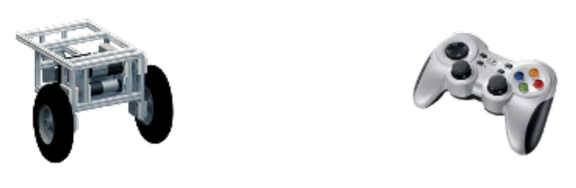
\includegraphics[]{robotandcontroller.pdf}
  \centering
\end{figure}
\newpage

\section{Kartierung mit GMapping}
Wir starten zuerst die Node zur Kommunikation mit dem Roboter: \begin{verbatim}
  roslaunch volksbot messtechnikpraktikum.launch
\end{verbatim}
Um den Roboter zu steuern mit dem Controller benötigen wir die zugehörige Node: \begin{verbatim}
  roslaunch volksbot localjoystick.launch
\end{verbatim}
Nun erstellen wir eine \textit{rosbag}, die alle Topics des Roboters aufzeichnet: \begin{verbatim}
  rosbag record -a
\end{verbatim}
Um nun eine Karte erstellen zu können, müssen wir die aufgenommene \textit{bag} abspielen. 
Wichtig hier ist es den Parameter \begin{verbatim}
  rosparam set use_sim_time true
\end{verbatim} zu setzen um die Zeit aus dem \textit{clock}-Topic zu nutzen anstelle der globalen Systemzeit.
Nun kann man aus den Laserscanner-Daten, also hauptsächlich dem \textit{LMS}-Topic, die Map
erstellen. Hierzu starten wir das GMapping-Tool via \begin{verbatim}
  roslaunch volksbot messtechnikgmapping.launch
\end{verbatim}
Die Bag kann dann abgespielt werden mit \begin{verbatim}
  rosbag play filename.bag --clock
\end{verbatim}
Der \textit{clock}-Befehl am Ende ist wichtig um die Aufnahmen der \textit{rosbag} mit einem 
Zeitstempel zu versehen damit der Roboter sie nicht verwirft. 
Startet man nun RViz kann man über das \textit{map}-Topic den Aufbau der Map betrachten.
Um diese zu speichern startet man eine \textit{ROS-node} die das \textit{map}-Topic in
eine Datei speichert. 

\begin{figure}[H]
  \caption*{Abbildung 2: Aufgezeichnete Karte des Informatik-Untergeschosses}
  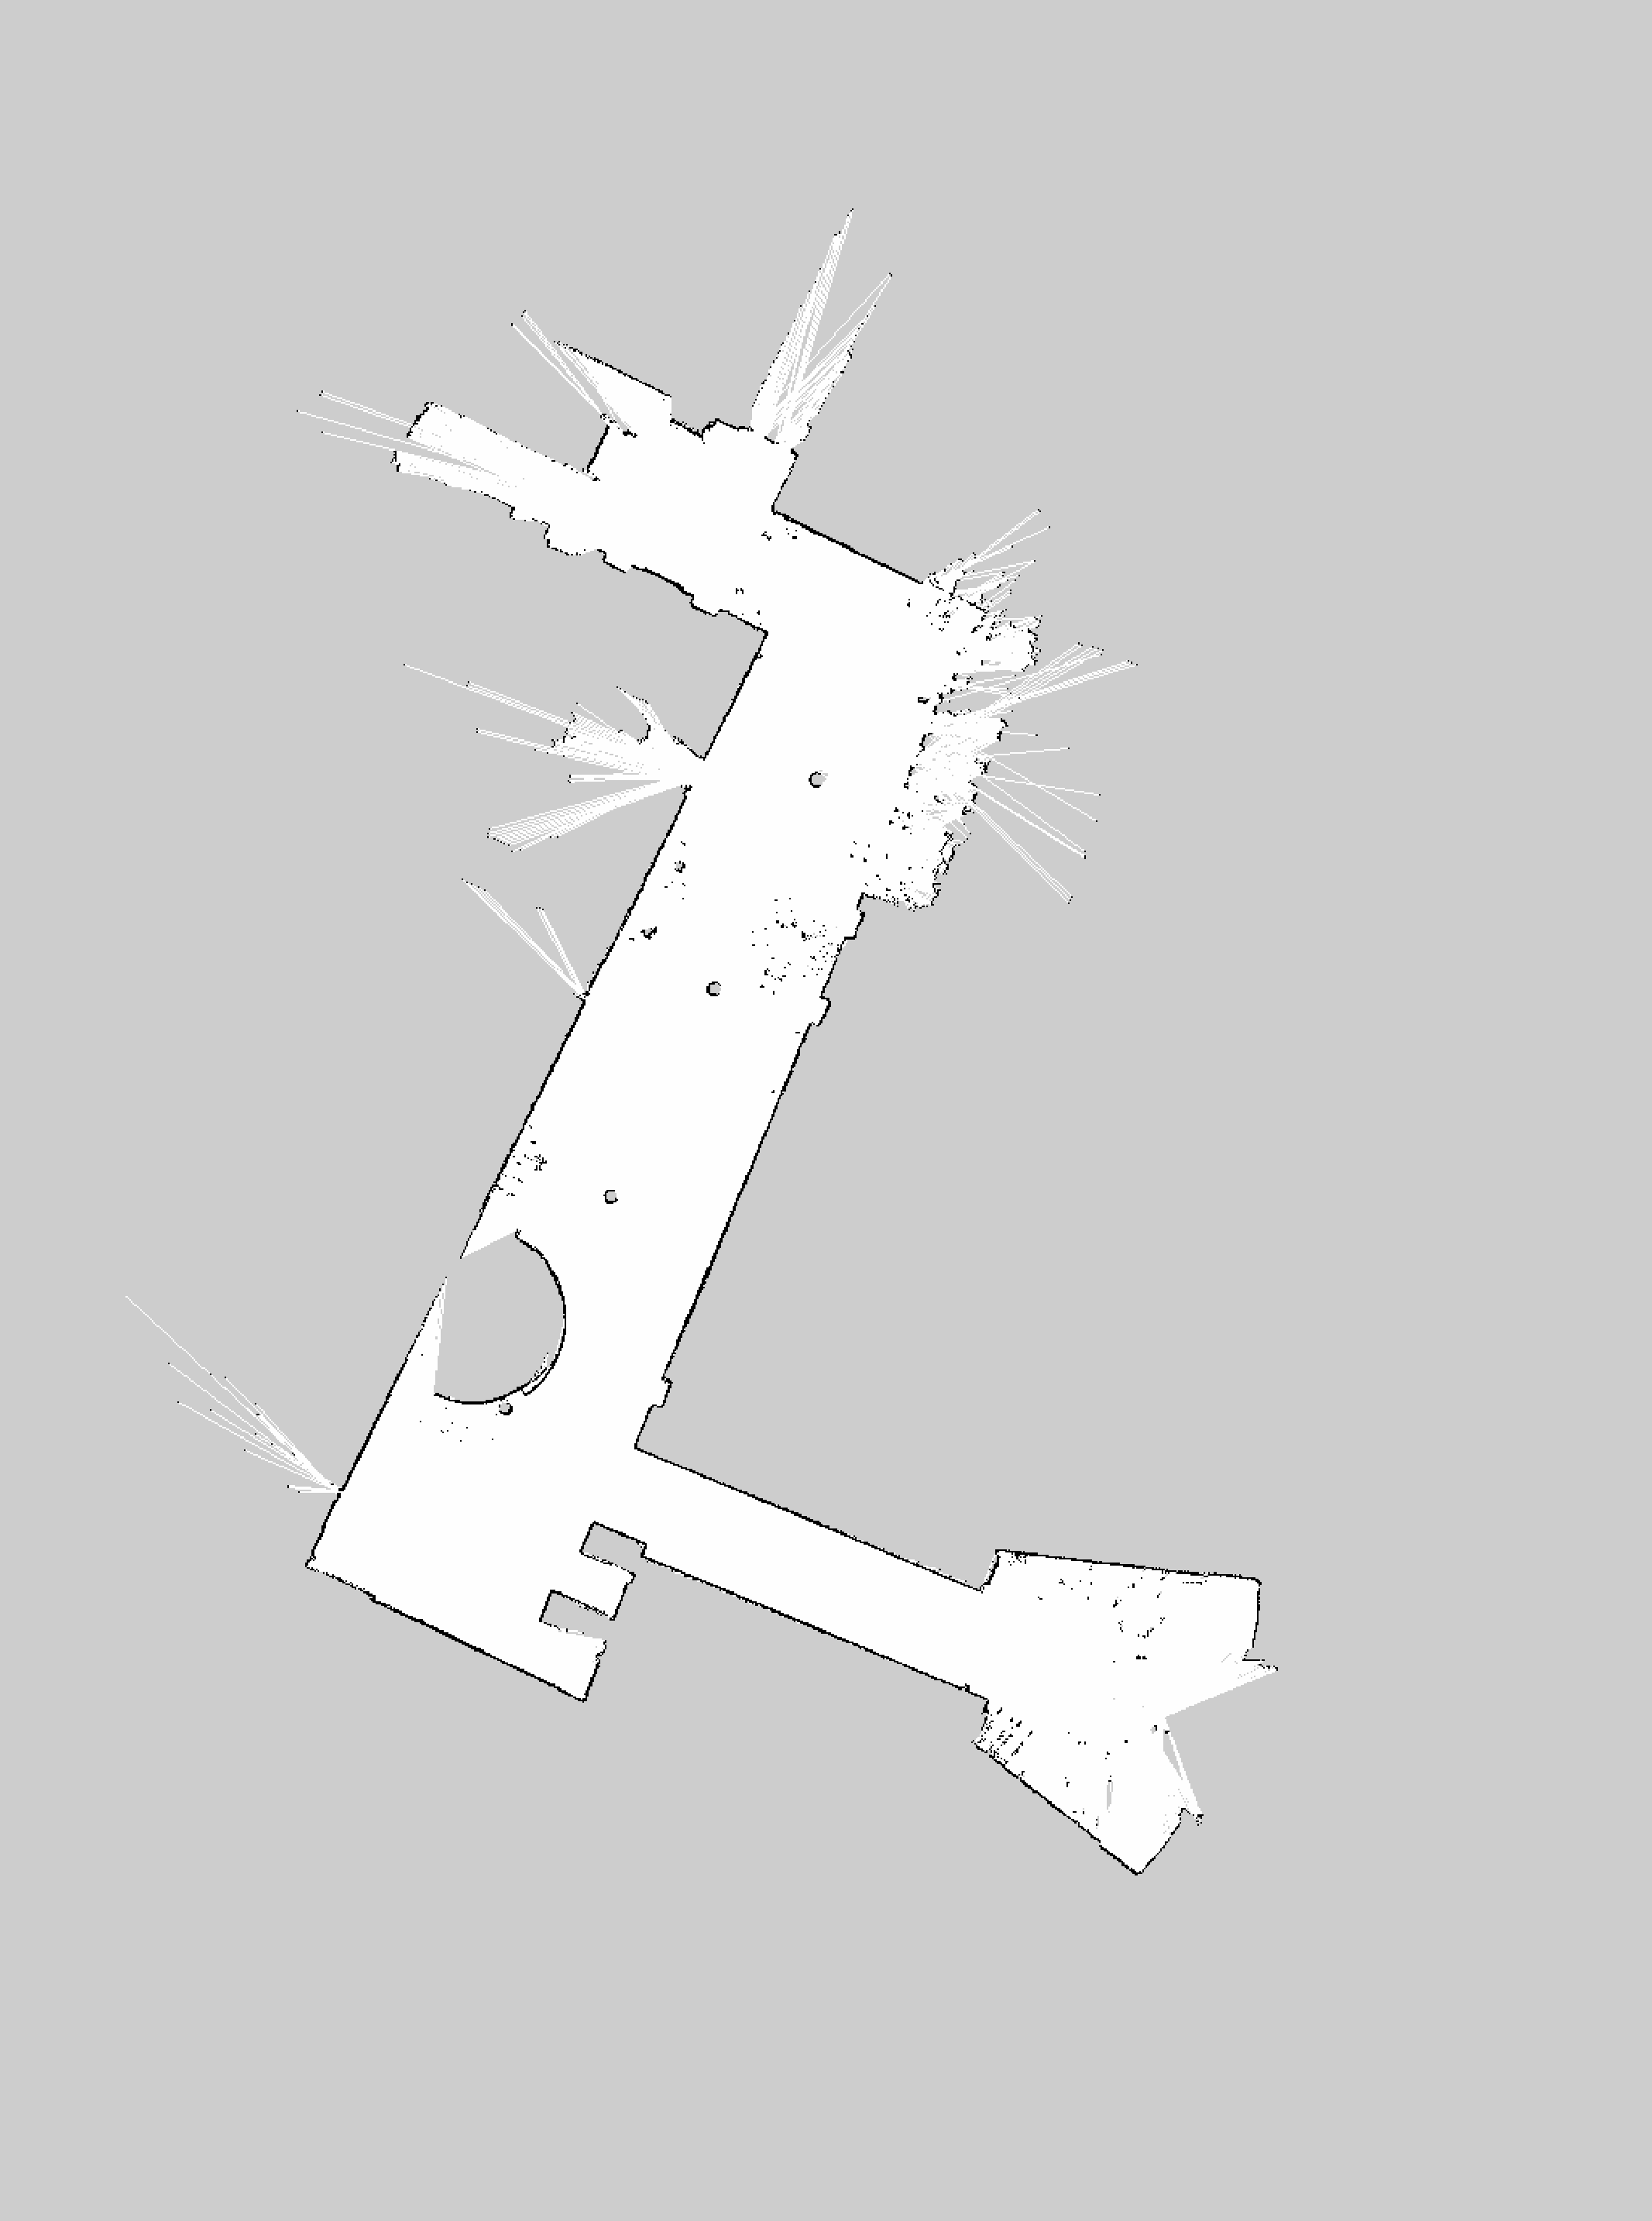
\includegraphics[scale = 0.3, angle = 90]{map.pdf}
  \centering
\end{figure}

% KOM: das ist falsch. zuerst fahren wir daten in eine Bag und machen aus der bag ne map
% KOM: wir brauchen dazu keine plots??? Wir haben nicht mal relevante. Ein bild der karte die wir rausbekommen haben reicht

\section{AMCL-Lokalisierung}
Um aus der Odometrie einen Pfad zu plotten erstellen wir ein eigenes ROS-Node. Das Node-Package heißt \verb|data_saver|, 
die Node an sich \texttt{listener}. Es ist Subscriber des Odometrie-Topics und speichert die empfangenen Daten 
in einer Datei im Format \verb|Xpos_Ypos| \\
Es hat zwei Modi, wie es diese Daten speichern kann:
\begin{center}
\texttt{rel}: Koordinaten im Pfad sind relativ zur Startposition des Roboters \\
\texttt{abs}: Koordinaten sind absolut aus dem AMCL-Frame \\
\end{center}
Man starte sie mit dem gewählten Modus:
\begin{verbatim}
  rosrun data_saver listener _mode := "abs || rel"
\end{verbatim}
Um AMCL zu starten nutzen wir die vorgegebene Launchfile:
\begin{verbatim}
roslaunch volksbot messtechnikamcl.launch
\end{verbatim}
Bei Betrachten des launchfile-Codes fällt auf dass zusammen mit dem AMCL-Node ein \verb|map_server|-Node gestartet
wird, welches eine vorgegebene Map published. Wir wollen aber unsere eigene Map verwenden, weswegen wir diese Zeile
auskommentieren und stattdessen eine eigene \verb|map_server|-Node starten, welches die Map aus \textit{GMapping}
published: \begin{verbatim}
rosrun map_server map_server map.yaml
\end{verbatim}
Außerdem muss im Configuration-File von AMCL noch eingefügt werden, dass AMCL auf ein Map-Topic subscriben soll,
und wie dieses Topic heißen soll. \\
In RViz muss man nun noch die Position des Roboters festlegen. Dazu setzt man die Map und das \verb|amcl_pose|-Topic
sichtbar, in unserem Fall mittels einer config-File, die man über \begin{verbatim}
rviz -d config.rviz
\end{verbatim}
ausführt.
In RViz drückt man nun den \verb|2D-Pose-Estimate|-Button, dann an die Stelle der Karte wo der Roboter am Anfang steht,
hält dabei gedrückt, und bewegt die Maus in die Richtung in die die Roboterlängsachse zeigt. Zum Bestätigen
lässt man den Mausbutton los. \\
Um die \texttt{rosbag}-Datei nun abspielen zu können, führe man folgenden Befehl im Terminal aus:
\begin{verbatim}
rosbag play file.bag --clock
\end{verbatim}
Der Roboter bewegt sich nun in RViz virtuell auf der Karte und lokalisiert sich dabei mit AMCL.

\begin{figure}[H]
  \caption*{Abbildung 3: RViz-Screenshot: Roboter lokalisiert sich in der Karte mittels AMCL}
  \includegraphics[scale = 0.25]{amcllocalisation.png}
  \centering
\end{figure}

\section{Pfadverfolgung}
\subsection*{Mit dem realen Roboter}
Elementar für die Pfadverfolgung ist das richtige Koordinatensystem sowie die richtige Referenz, in unserem Fall $absolut \leftrightarrow relativ$ \\
Die Punkte des Roboters liegen in einem anderen System als die gegebenen Pfade, daher müssen
wir die Position des Roboters in dieses System transformieren, wenn wir diese Pfade verwenden wollen. 
Für absolute Pfade ist dies nicht nötig, da die Koordinatensysteme bereits zueinander passen. 
Wir geben diese Position an den Controller weiter und publishen dann die Ausgaben des Controllers auf dem 
selben Topic auf dem auch unser Joystick-Controller die Steuerbefehle an den Roboter weitergibt. 
Wir legen mit einer Modiswitch fest ob AMCL oder Odometrie verwendet werden soll. Die AMCL-Node muss 
bei Bedarf separat zugeschaltet werden und wird bei unserem Pfadverfolgungs-Code nicht mit aufgerufen.
Die node startet mit \begin{verbatim}
rosrun robo_pathing robo_drive _file="file"_mode:="amcl || odom"_coord:="rel || abs"
\end{verbatim}
Für AMCL (\textit{if required}):
\begin{verbatim}
roslaunch volksbot messtechnikamcl.launch
\end{verbatim}
Wir benutzen den Pfad aus unserer \verb|data_saver|-AMCL-Node im \texttt{abs}-mode als Datei
für das \verb|robo_drive.cpp|-Node zum Abfahren mit dem Volksbot. Dies ist im AMCL-\texttt{"abs"}-Mode. \\
Als Terminalbefehl sieht dies dann folgendermaßen aus:
\begin{verbatim}
rosrun robo_pathing robo_drive_file:="mapaufnahmenAMCL.dat"_mode:="amcl"_coord:="abs"
\end{verbatim}

\subsection*{Simulation}
Der Code der aus der Position des Roboters und der Position des nächsten Punkts die Rad-geschwindigkeit ausgibt
ist bereits gegeben. Wir müssen die Bewegung des Roboters nach einem Zeitschritt $\Delta t$ simulieren.
Unser Ansatz dabei ist: Wenn die Winkelgeschwindigkeit des Roboters größer als ein Schwellenwert ist, fährt der Roboter einen 
Kreisausschnitt, angefangen an seiner momentanen Position. Die Endposition daraus berechnen wir und
geben sie an den Controller zurück. Wenn die Winkelgeschwindigkeit kleiner ist als der Schwellenwert
approximieren wir die Bewegung mit einer geraden Linie. Der Code dazu befindet sich in der Datei \verb|robo_simu.cpp|.
Wir übergeben den zu fahrenden Pfad als Parameter. Die ROS-Node startet dann mit \begin{verbatim}
rosrun robo_pathing robo_simu _file:="file"
\end{verbatim}
\newpage

\section{Auswertung}
Insgesamt fällt auf dass sich die Fehler bei der Odometrie aufaddieren, während sich die Fehler für die AMCL-Lokalisierung
auf einem gleichen Level über den gesamten Pfadverfolgungszeitraum bewegen. Der Grund dafür liegt in der fehlenden Korrektur der Odometriedaten, die 
nicht die Reibung der Reifen oder das Rutschen des Roboters bei schnellen Änderungen der Radgeschwindigkeiten und der Richtung korrigieren können und nur über Iteration die Position bestimmen.
\begin{figure}[H]
    \caption*{Abbildung 4: Pfadaufnahme der Karte mittels Odometrie, Einheit [m]}
    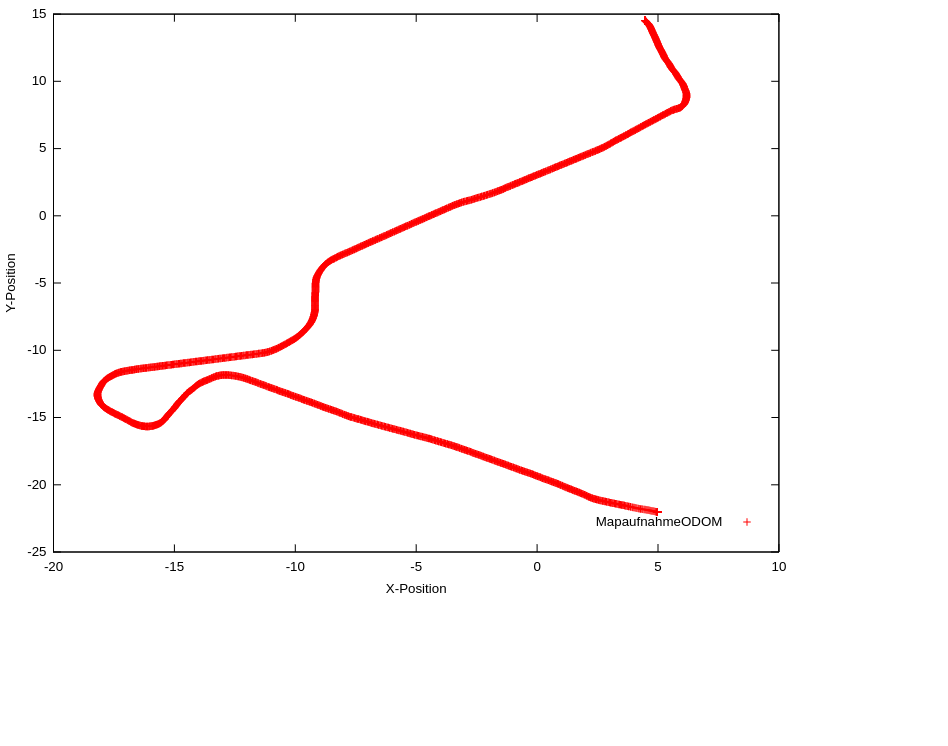
\includegraphics[scale = 0.6]{Plots/better ones/mapaufnahmeODOM.png}
    \centering
\end{figure}
\vspace{-25mm}
Hier liegt die Stärke von AMCL, da die Positionsbestimmung einem konstanten Fehler unterliegt, der zwar anfangs größer sein kann als der der Odometrie,
sich aber über längere Zeiträume dafür nicht aufaddiert und über weite Strecken konstant bleibt. Bei kleinen Pfadabständen zu Hindernissen kann die Summe der Odometriefehler dazu führen dass 
der Roboter den vorgegebenen Pfad nicht mehr abfahren kann und an Hindernissen hängen bleibt.
\begin{figure}[H]
    \caption*{Abbildung 5: Pfadaufnahme der Karte mittels AMCL, Einheit [m]}
    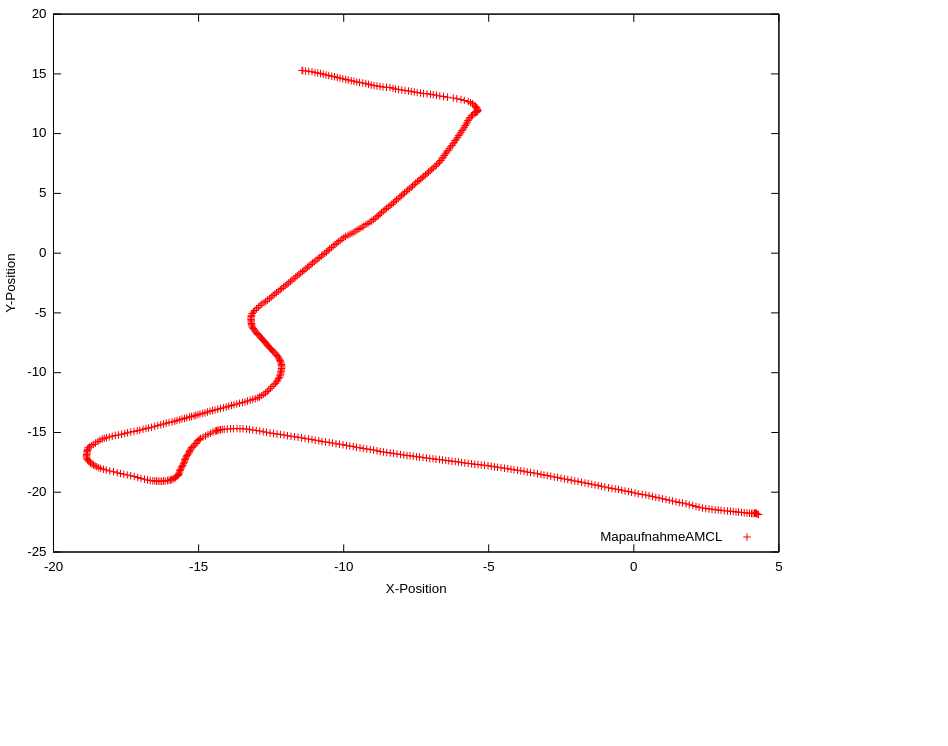
\includegraphics[scale = 0.6]{Plots/better ones/mapaufnahmeAMCL.png}
    \centering
\end{figure}
\vspace{-25mm}

Die Stärke der Odometrie liegt in Fahrten die die oben genannten Fehler klein halten, z.B. ein langsames Abfahren eines Pfades mit wenig Kurven.

\subsection*{Vergleich der Fahrten mit Odometrie und AMCL}
\begin{figure}[H]
  \caption*{Abbildung 8: Realer Pfad des Roboters unter Verwendung von AMCL, angedeutet mit farbigen Streifen für das rechte und linke Rad des Roboters}
  \includegraphics[scale = 0.25]{AMCLAcht.png}
    \caption*{Abbildung 9: Realer Pfad des Roboters unter Verwendung von Odometrie, angedeutet mit farbigen Streifen für das rechte und linke Rad des Roboters}
    \includegraphics[scale = 0.25]{odomAcht.png}
    \centering
  \end{figure}

Wir ließen den Roboter eine Acht jeweils unter der Verwendung von AMCL/Odometrie-Lokalisierung nachfahren. Dabei modifizierten wir den driving code sodass der Roboter alle 3 Sekunden anhält,
um Zeit zu haben den Pfad des linken und rechten Rades zu markieren. Die Bilder sind nachbearbeitet um diese besser sichtbar zu machen. Auch wurde die Startposition mit roten, die Endposition mit 
weißen Strichen markiert. Es ist zu erkennen, dass diese bei der Verwendung von AMCL deutlich näher beinander im  Vergleich zum Odometrie-Fall. Idealerweise sollten sie exakt aufeinander liegen, denn so ist 
der Pfad beschrieben. Dass sie dies nicht tun liegt zum einen daran, das im Code des Giovanni-Controllers der Pfad schon als vollständig erachtet wird wenn man in kurzer Reichweite des letzten anzufahrenden Punktes ist.
Da wir den Roboter auf der schwarzen Linie, mit einer Ausrichtung im rechten Winkel zu dieser haben starten lassen, sollte diese bei idealer Pfadverfolgung die Symmetrieachse der Acht darstellen. Leider sind die Bilder durch
unsere Aufnahmemöglichkeiten etwas verzerrt, jedoch ist noch gut zu erkennen dass Dies bei AMCL sehr viel mehr der Fall ist als bei der Odometrie-Lokalisierung, wo der Großteil der unteren Hälfte der Acht auf der linken Seite 
der schwarzen Linie liegt. Schon aus dieser groben Betrachtung kann schließen wir dass die AMCL-Lokalisierung deutlich besser in der realen Welt funktioniert als Odometrie.

\begin{figure}[H]
  \caption*{Abbildung 6: Abfahren einer liegenden Acht mit AMCL, Einheit [m]}
  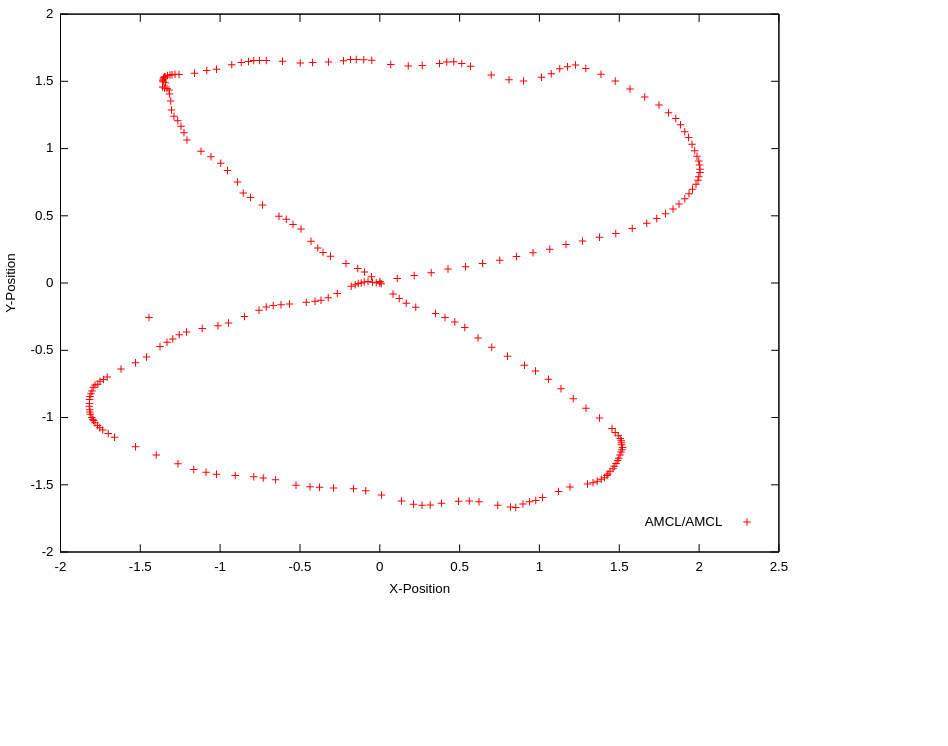
\includegraphics[scale = 0.45]{Plots/better ones/amclamclacht.png}
  \vspace{-20mm}
\\ Dies ist ein Plot der Position aus der AMCL Lokalisierung während der Roboter mit diesen Daten eine Acht abfährt.
  \caption*{Abbildung 7: Abfahren einer liegenden Acht mit Odometrie, aufnehmen der Position anhand der AMCL Lokalisierung, Einheit [m]}
  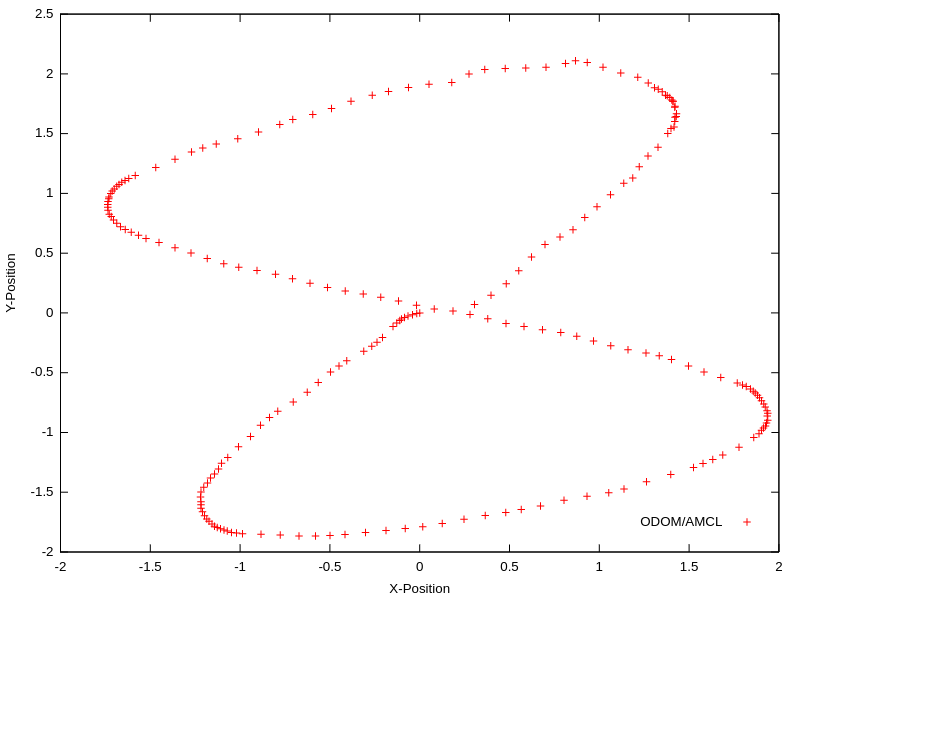
\includegraphics[scale = 0.45]{Plots/better ones/odomamclacht.png}
  \vspace{-20mm}
\\ Dies ist ein Plot der Position aus der AMCL Lokalisierung während der Roboter anhand der Odometrie eine Acht abfährt. Wie vorher erörtert können wir die AMCL-Lokalisierung als gutes analog zur Position in der echten Welt verwenden. 
Man erkennt einen deutlichen Unterschied zum vorherigen Plot, vorallem dass hier die Start- und Endposition weniger übereinstimmen.
  \centering
\end{figure}

% KOM: An Plots brauchen wir hier Simulation, den rohen Pfad, AMCL, Odom, und Bilder was er IRL jeweils getan hat. Die Bilder kann ich noch machen.



\end{document}

